%!TEX root = /Users/markelikalderon/Documents/Git/timaeus/timaeus.tex

\chapter{Cognitive Revolution} % (fold)
\label{cha:cognitive_revolution}

\section{Psychogeny and Cognitive Power} % (fold)
\label{sec:psychogony_and_psychic_power}

The psychogony, understood strictly as Timaeus' account of the generation of the World Soul, was the topic of the last chapter. Timaeus' account of the generation of the World Soul is important since the nature of its substance, its proportional division, and its structure determine its kinetic and cognitive powers. Our understanding of these powers is incomplete unless they are understood to be determined, at least in part, by the substance, proportional division, and structure that the World Soul has thanks to Demiurgic activity. The details of the Demiurge's manufacture and construction of the World Soul thus go some way toward explaining the powers that He invests it with. Timaeus makes this connection explicit with respect to its cognitive powers. The World Soul has its cognitive powers inasmuch as it is a mixture of indivisible and divisible forms of Being, Sameness, and Difference, proportionally divided, and revolves around itself (37a). The explanation of World Soul's cognitive powers would thus involve its substance, proportional division, and structure.

The World Soul is an elder sister to the souls of mortal beings. The Demiurge is the Maker and Father of the World Soul as well as the souls of mortal beings. The World Soul and souls of mortal beings are thus siblings. The souls of mortal beings are generated after the generation of the World Soul. The souls of mortal beings are thus younger siblings to their elder sister, the World Soul. Moreover, just as siblings share the blood of their parents, the World Soul and the souls of mortal beings share a substantial nature. The souls of mortal beings are mixed from the same material, though impurely, that was used to mix the substance of the World Soul. Moreover, the Demiurge invests the souls of mortal beings with the same proportional divisions and structure as the World Soul. The World Soul is prior not only in birth but in dignity. It is more perfect than the souls of mortal beings as signaled by the impurity of their substance. Being perfect it is an exemplar for the souls of mortal beings. Thus like an elder sister, the souls of mortal beings look to her for guidance. Literally. The cognitive powers of the World Soul are visibly manifest in the harmony of celestial motion. And by watching this motion and rationally attending to it in the right sort of way the circles in the souls of mortal beings are aligned to the circles in the World Soul making them more rational and virtuous. We should all strive to follow the good example set by our elder sister.

The way that the psychogony explains the exercise of the cognitive powers of the World Soul is relevant to the psychology of mortal beings. Given the relationship between the World Soul and the souls of mortal beings, the explanation of powers of the souls of mortal beings should parallel the explanation of the powers of the World Soul. That is not to deny that there will be differences. The World Soul and the souls of mortal beings differ:
\begin{enumerate}[(1)]
	\item in the purity of their substantial mixture (the souls of mortal beings are composed of the same mixture, if less pure, as the World Soul),
	\item in the character of their soul--body union (the World Soul encompasses the body of the Cosmos whereas the souls of mortal beings are encompassed by the bodies they animate), and
	\item in the waverability of their revolutions (whereas the revolutions of souls of mortal beings are waverable, the revolutions of the World Soul are not).
\end{enumerate}
These and other differences leave open the possibility, consistent with the explanatory parallels, that the cognitive activity of the souls of mortal beings differs from the cognitive activity of the World Soul. (1) The impurity of the mixture that composes the substance of the souls of mortal beings may impair its motion and activity. (2) If one is unclear how a difference in the soul--body union could make for a difference in cognitive activity, consider how these souls are differently related to the sensible and the corporeal. In encompassing the sensible and the corporeal, the sensible and the corporeal are endogenous to the World Soul whereas they are exogenous to the souls of mortal beings. And this plausibly makes a difference to the way in which the sensible and corporeal are cognitively accessed by each. (3) While the souls of mortal beings are embodied and embedded in an environment with strong powers, the World Soul, while embodied, is not. Since they are embodied and embedded in an environment with strong powers, the revolutions of the souls of mortal beings are affected from without by linear motion of \emph{aisthēsis}. Since the body of the Cosmos as animated by the World Soul is not embedded in an environment, it is not subject to the effects of strong powers. The revolutions of the World Soul are thus not affected from without in this way. The revolutions of the World Soul are thus not waverable in the way that the revolutions of the souls of mortal beings are. The parallels and differences begin to make sense once we realize that the cognitive powers and activities of the World Soul are epistemically ideal in the way that the cognitive powers and activities of the souls of mortal beings are not.

This chapter will discuss the cognitive powers of the World Soul as Timaeus presents them to be at 37a--c. The passage consists in two long and syntactically complex sentences that have been variously interpreted. There Timaeus describes:
\begin{enumerate}[(1)]
	\item The substantial mixture, proportional division, and structure of the World Soul as enabling its cognition
	\item The World Soul's ``contact'' (\emph{ephaptētai}) with its objects
	\item The objects of these cognitive powers, divisible and indivisible beings
	\item The cognitive activity that ``contact'' (\emph{ephaptētai}) elicits
	\item The two kinds of cognitive powers that the World Soul enjoys, the power to understand (\emph{nous}) and know (\emph{epistēme}) and the power to have true opinion (\emph{doxa}) and conviction (\emph{pistis}).
\end{enumerate}
We shall consider each of these for the most part in order of their occurrence in Timaeus' speech. However, to facilitate exposition, we shall begin with the objects of cognition.

% section psychogony_and_psychic_power (end)

\section{The Objects of Cognition} % (fold)
\label{sec:the_objects_of_cognition}

The objects of cognition have either divisible or indivisible Being. Divisible Being is associated with Becoming (\emph{gignomenēs}) and is divided around bodies (\emph{peri ta somata} \ldots\ \emph{meristēs}), whereas indivisible Being always remains the same (\emph{aei kata tauta}). Being divided around bodies, divisible Being is corporeal in the sense that divisible Being is the kind of Being suffered by bodies. And since the sensible is the mark of the corporeal, divisible beings are sensible. Indivisible Being, by contrast, are not divided around bodies, and so are not sensible and corporeal, but are, rather, intelligible.

How is this related to the psychogony? Timaeus specifies the different kinds of objects of cognition in terms a difference in their Being. One kind enjoys indivisible Being, and the other suffers divisible Being. Being is mixed into the substance of the World Soul. And though Timaeus does not make this explicit in his summary statement of the soul mixture at 37a, this involved mixing indivisible and divisible Being. That the substance of the World Soul consists in a mixture of divisible and indivisible Being perhaps explains, at least in part, that the objects of its cognition are either divisible or indivisible beings. If so, perhaps Timaeus subscribes, as Aristotle (\emph{De anima} 1.2 404b16--18, 1.3 406b28--31, Alcinous \emph{Didaskalikos} 14.4) suggests, to some version of the principle that like is known by like. How that principle is best interpreted shall be clarified as we proceed.

It will emerge that the World Soul has different cognitive powers. On the one hand, the World Soul understands (\emph{nous}) and knows (\emph{epistēme}) and, on the other hand, the World Soul has true opinion (\emph{doxa}) and conviction (\emph{pistis}). How do the two objects of cognition relate to the two cognitive powers? A traditional interpretation has it that the World Soul understands (\emph{nous}) and knows (\emph{epistēme}) indivisible beings and it has true opinion (\emph{doxa}) and conviction (\emph{pistis}) about divisible beings. The stability of indivisible beings, that they always remain the same, make them appropriate objects of knowledge. Whereas the instability of divisible beings, belonging to the realm of Becoming, makes them at best the objects of true opinion. This interpretation has been challenged, however, by \citet{Frede:1996rb} and \citet{Corcilius:2018bd}. We shall return to this question when we discuss The World Soul's powers of knowledge and opinion.

% section the_objects_of_cognition (end)

\section{Substantial Mixture, Proportional Division, and Structure} % (fold)
\label{sec:the_substantial_mixture_proportional_division_and_structure_of_the_world_soul}

Timaeus explains why the World Soul has its cognitive powers in terms of its substantial mixture, proportional division, and structure. He explicitly signals this with his use of the causal \emph{ate} (37a2). Paraphrasing, Timaeus says that since (\emph{ate}) the World Soul has been (1) mixed from Being, Sameness and Difference, (2) proportionally divided and bound, and (3) circled back upon itself, then whenever it applies itself to divisible and indivisible beings, it moves throughout its whole self and declares the same as the same and the different as different. Timaeus, here, is conceiving of cognitive activity on the model of inner speech. How does the
\begin{enumerate}[(1)]
	\item substantial mixture,
	\item proportional division, and
	\item structure
\end{enumerate}
of the World Soul explain its power to engage in discursively structured activity? Let us briefly review each of these three features.

(1) \emph{Substantial mixture}. How does being composed of a mixture of Being, Sameness, and Difference help explain the cognitive powers of the World Soul? Recall (chapter~\ref{sec:soul_mixture}), though Timaeus does not mention this in his summary statement, the Demiurge mixes indivisible and divisible forms of Being, Sameness, and Difference. The Demiurge proceeds in two stages. First He mixes indivisible and divisible forms of each to generate intermediary forms of Being, Sameness, and Difference. Then He mixes these intermediary forms of Being, Sameness, and Difference. It is from this final mixture that the Demiurge constructs the World Soul. This is worth reminding ourselves of since the objects of cognition turn out to be divisible and indivisible beings. It is reasonable to conjecture that the World Soul is capable of cognizing both divisible and indivisible beings, at least in part, because it is itself composed of divisible and indivisible Being. This would be to understand the causal \emph{ate} as being underwritten by the principle that like is known by like (Aristotle, \emph{De anima} 1.2 404b16–18, 1.3 406b28–31, Alcinous, \emph{Didaskalikos} 14.4).

A problem arises when we try to extend this explanation to the cognition of sameness and difference. Perhaps the World Soul may cognize divisible and indivisible beings by being composed, in part, of divisible and indivisible forms of Being. But the objects of cognition do not seem to be composed of Sameness and Difference the way that the World Soul is. Difference is not an element in the composition of divisible and indivisible beings. Sameness and Difference are not aspects of how things are in themselves but how they are in relation to either themselves or other things. Sameness and Difference thus contrast with Being \citep[58--9]{Corcilius:2018bd}. The World Soul may be composed of the kind of Being that its objects have, but these objects do not have Sameness and Difference \emph{simpliciter} but only in relation to one another and in certain respects.

\citet{Corcilius:2018bd} argues that this is less an objection to the principle that like is known by like than to a certain ``archaic'' interpretation of it. On that interpretation, like is know by like is interpreted in terms of substantial similarity. Consider the Empedoclean fragment cited by Aristotle:
\begin{verse}
	By earth we see earth; by water, water;\\
	by aither, shining aither; but by fire, blazing fire;\\
	love by love and strife by baneful strife (Empedocles DK 31B109; \citealt[221]{Inwood:2001ve})
\end{verse}
On the most straightforward understanding of this passage, we perceive earth, at least in part, by being composed of earth. The likeness that explains the exercise of our perceptual powers is a substantial likeness. It is because we are composed of earth that we can come to perceive objects that are themselves composed of earth. If Timaeus does in fact subscribe to the principle that like is known by like, even in explaining the World-Soul's cognition of the sameness and difference of divisible and indivisible beings, then the principle must be interpreted in some other way than in terms of substantial similarity.

(2) \emph{Proportional divisions}. Not only is the mixture explanatorily relevant to the World Soul's cognition but so is its proportional division. Specifically, Timaeus says that the World Soul cognizes because the mixture from which its substance is composed is proportionally divided and bound. This claim can be understood in terms of the account of soul mixture we gave in chapter~\ref{sec:proportional_division}. The mixture is divided since drawing from the \emph{krater}, the Demiurge linearly apportions the mixture. The magnitudes of the portions of soul mixture stand in various proportions. And these portions are held together by the proportions in which they stand, proportion being the fairest and most perfect of bonds (31c2--4).

What is the cognitive significance of proportional divisions and bonds so understood? The World Soul's cognition is discursive, and a discursive act is divided. Only so may it display discursive structure. Discursive acts are not merely divided. Not every plurality of words constitutes a meaningful statement (\emph{Sophist} 263d). To make a meaningful statement, the speaker must ``weave'' together a noun and a verb (\emph{Sophist} 262d4). While discursive acts must be divided in order to display discursive structure, they must also be bound together in order to intelligibly occur. Suppose that the proportional divisions in the substance of the World Soul make possible distinct activities or aspects of activities. If sufficiently complex, these may display discursive structure, but only when harmoniously related and so bound by proportion.

(3) \emph{Structure}. Not only is the substantial mixture and its proportional divisions and bonds explanatorily relevant to the World Soul's cognition, but so is its structure. In speaking of structure, here, I have already offered an interpretation. Timaeus speaks of the mixture proportionally divided and bond as revolving back upon itself. A natural interpretation is to understand TImaeus to be speaking of the circular motion or activity of the World-Soul. However, there is a problem with this reading. The motion of the World Soul is at the very least closely related to its discursive cognitive act if indeed they are not identified. If they are indeed identified, then motion is the \emph{explanandum} not the \emph{explananda} and should not occur in the causal \emph{ate} clause. 

The mixture proportionally divided and bound revolving back upon itself need not be read as the revolution of the World Soul. It can be read as describing, not the World-Soul's circular motion, but its circular shape. Specifically, the Demiurge, having placed the two strips of soul mixture center to center and at oblique angles, bends these strips back upon themselves to form outer and inner circles, the Circles of the Same and the Different. The mixture proportionally divided and bound revolving back upon itself may be read as an impersonal description of its being shaped into the Circles of the Same and the Different. So understood, what is explanatorily relevant to the World Soul's cognition is its structure, its being shaped into the Circles of the Same and the Different. Since they are circular, not only are they capable of circular motion but they may revolve within their own limits (\emph{en tō autō}). (A cube may rotate and so engage in circular motion and yet fail to revolve within its own limits.) And Timaeus regularly links thought with circular motion within its own limits. On the present interpretation, then, the structure of the World Soul is explanatorily relevant to its cognition, since it makes possible its circular motion within its own limits, which either is its cognitive activity or is closely related to it.

% section the_substantial_mixture_proportional_division_and_structure_of_the_world_soul (end)


\section{\emph{Ephaptētai}} % (fold)
\label{sec:_emph_ephatetai}

The World Soul is in ``contact'' (\emph{ephaptētai}) with the objects of cognition, be they divisible or indivisible, sensible or intelligible. As a result of this, the World Soul is moved throughout the whole of its being and so announces what it is in contact with. How one understands \emph{ephaptētai} potentially constrains how one understands the motion of the World Soul throughout the whole of its being by which it announces the object of its cognition. It is worth reflecting upon the meaning of the occurrence of this verb. (In the Platonic corpus, \emph{ephaptētein} also occurs at \emph{Res Publica} 7 534c5, 10 598b8, \emph{Timaeus} 71e3, \emph{Leges} 3 682a5, \emph{Epistulae} 7 343e7)

So far I have followed the bloodless convention of translating the verb \emph{ephaptētai} as a kind of contact. That verb, however, has a range of uses. The different senses conveyed by these may prove relevant. Let us begin by reviewing at least some of them.

In a range of uses the verb is used to convey \emph{binding}, somehow \emph{fixing} or \emph{holding fast} (Homer, \emph{Odyssey} 22 41). Observe that the emphasis is on the activity of binding rather than on the state of being bound. In another range of uses the verb has more tactile associations. It may be used to convey \emph{reaching} (Euripides, \emph{Helen} 556) or \emph{laying hands on} (Homer, \emph{Odyssey} 5 348). This second range of uses also emphasizes the activity of the subject of the verb. Reaching and laying hands on are bodily activities. They are something done by embodied mortal beings embedded in an environment. They \emph{apply themselves} to that environment (Pindar, \emph{Olympian} 1 186). Moreover, reaching is an exploratory activity in a way that laying hands on may at least sometimes be (\citealt[134]{Betegh:2019fq}, emphasizes this aspect of \emph{ephaptein}'s usage). The senses associated with these different uses need not conflict. Indeed, they may combine. Thus, for example, \emph{grasping} involves reaching and is a way to lay hands on something, but it also binds what is in its grasp. The verb has gustatory uses that emphasize not binding so much as assimilation, as when one \emph{partakes} of food (Iamblichus, \emph{Vita Pythagorae} 3 17). The verb also has purely cognitive uses that designate a kind of cognitive \emph{apprehension} (Plato, \emph{Symposium} 212a). (For discussion of a similar semantic field associated with perceptual apprehension see \citealt[chapters 1--2]{Kalderon:2018oe}.)

\citet[]{Corcilius:2018bd} observes a similar pattern in Timaeus' use of the root of the verb, \emph{haptein}:
\begin{quote}
	We can distinguish two main uses of `\emph{haptein}' and its compound forms in the dialogue. First, it is used in the sense of `attaching', `bestowing on', `binding things together' (33 D 5; 37 D 4; 75 D 5). This seems to imply a literal understanding of `contact' (reciprocal contiguity) and hence seems irrelevant to our case. Second, it is used in the sense of `having some grasp' (52 B 2; 71 E 1, 3; 90 C 2). \citep[85]{Corcilius:2018bd}
\end{quote}
As Corcilius goes on to explain, \emph{having some grasp} is a generic kind of cognitive apprehension that admits of distinct species.

\citealt{Corcilius:2018bd} and \citet[]{Betegh:2019fq} have argued that the present occurrence of \emph{ephaptētai} must itself be understood in an active sense. The usual bloodless translation where the World Soul is in contact with divisible and indivisible beings obscures the activity conveyed by the Greek. The World Soul instead applies itself to divisible and indivisible beings. Even if one thought that \emph{ephaptein} involved corporeal contact, its active character would be better captured by translating the verb as touching or reaching out and grasping.

The range of senses associated with \emph{ephaptein} are all potentially cognitively significant. Reaching out and grasping would be an apt metaphor for the World Soul's cognitive apprehension of divisible and indivisible being. Cognitive apprehension is the World Soul's activity, the way grasping is an activity. And, insofar as the object is apprehended, it is apt to think of this as a kind of binding, as when something is bound in one's grasp. And this remains true even when the binding could not be corporeal the way a grasping must be. Perhaps there are echoes of the other senses as well. The soul, in thinking, applies itself to the object of thought. Perhaps the soul, in applying itself to divisible or indivisible beings, assimilates to these. In applying itself to the object of thought the soul partakes of what it thinks and becomes like it, in some suitable sense. This might be manifest in the ethical challenges that Timaeus understands the sensible to pose (90b). And Timaeus' sensory soteriology presupposes something like the mortal soul' ability to assimilate to the object of its contemplation (46e--47e). The Young Gods, acting on the Demiurge's behest, providentially provide mortal beings with eyes to see with. In rationally attending to the harmony of celestial revolutions, the mortal being may align the circles in their soul with the circles in the World Soul. Providentially provided sight is a means of salvation only insofar as it is a means by which the souls of mortal beings may assimilate to the soul of a divine immortal being and so become like their elder sister, insofar as possible.

To understand what \emph{ephaptētai} means in this context, let us begin by considering an obvious hypothesis about a special case. Begin by considering the case where the World Soul applies itself to a divisible being and, hence, to something sensible and corporeal. Since the object of cognition is sensible and corporeal, it is natural to consider whether \emph{ephaptētai} might involve a kind of corporeal contact. The tactile imagery conveyed by some uses of the verb---reaching, laying hands on---may suggest this. (Aristotle, \emph{De anima} 1.3 407a, reads Timaeus this way, for discussion see \citealt[392--5, 404--7]{Cherniss:1944aa} and \citealt[82--6]{Lee:1976xs}.) Just as a body may set into motion another body by coming into contact with it, perhaps the sensible and corporeal object of cognition sets the World Soul into motion in just the same way. When the World Soul applies itself to its corporeal object, this causes it to move throughout its whole being. The World Soul is said not merely to move, but to move throughout its whole being. How are we to understand this qualification? The World Soul, though incorporeal, is conceived as a voluminous sphere. Perhaps circular motion such as axial rotation would be a way for a voluminous sphere to move throughout its whole being. Beginning with our assumption that \emph{ephaptētai} involves corporeal contact, we were led to conceive of the resulting motion as the axial rotation of a voluminous sphere. This could only be so if the World Soul were spatial. Only spatial things are spherical. Importantly, the World Soul is also set into motion as a result of its contact with the divisible being, making the axial rotation subject to mechanical explanation.

There are difficulties in understanding \emph{ephaptētai} as corporeal contact, however. Let us consider two such difficulties. The first concerns the location of the object of cognition and the second concerns the mechanical explanation of the motion of the World Soul.

The first difficulty concerns the location of the object of cognition. Aristotle (\emph{De anima} 1 3 407a) understands the Circle of the Different coming into contact with a divisible being at a point or segment of its circumference. The circles in the soul in this way touch their objects. So understood, the object of cognition would be located at the circumference of the circle. This, however, seems to fundamentally misunderstand the cognitive significance of circular motion. Specifically, Aristotle fundamentally misunderstands how the object of cognitive activity is represented in the \emph{eikōs muthos}. As we shall see (section~\ref{sec:the_cognitive_significance_of_circular_motion}), Timaeus has transformed an Eleatic pun where what the circle revolves about (\emph{peri}), its center, is what the thought is about (\emph{peri}), its object. Notice that the Eleatic pun locates the object of cognition, not at the circumference of the circle but at its center. This is what allows the use of \emph{peri}, with its spatial connotations of being around or about, to be used to specify the object of cognitive activity. The object of cognition is at the center of cognitive activity not at its periphery (see figure~\ref{fig:center_periphery}).

\begin{figure}[htbp]
	\centering
		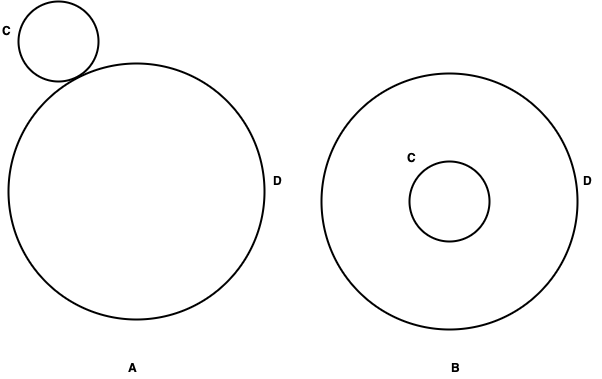
\includegraphics[scale=0.4]{graphics/center_periphery.png}
	\caption{A = the relationship between the object of cognition and the circle of the soul that Aristotle attributes to Timaeus, B = the relationship between the object of cognition and the circle of the soul as Timaeus in fact conceives of it, C = the object of cognition, D = the circle of the soul}
	\label{fig:center_periphery}
\end{figure}

Another difficulty concerns the mechanical explanation of the motion of the World Soul. The mechanical explanation requires the corporeal object to be solid and offer resistance, and the incorporeal soul to itself be solid in order to be moved by contact with the corporeal object (\citealt[129--33]{Betegh:2019fq}). The potential problem is that solidity, on some understanding of that notion, is a condition on the possibility of touch (see chapter~\ref{sec:the_elemental_composition_of_the_corporeal}). If the solidity of the extended if incorporeal soul is suitably understood, then while the World Soul may be invisible, it is tangible. When Timaeus claims that the World Soul is invisible (36e), does he allow for this? Is it really plausible that the World Soul may be felt if unseen? Or is invisible (\emph{aoratos}) an exemplar for insensible, in which case the World Soul is intangible? That Timaeus takes visibility and tangibility to be opposed extremes of the sensible provides some support for the more general reading (Proclus, \emph{In Timaeum} 2 6--7, \citealt{Diehl:1903re}, see also Calcidius' translation of 31c as well as his \emph{In Timaeum} 21, discussed in chapter~\ref{sec:the_elemental_composition_of_the_corporeal}). If the World Soul is insensible, it is intangible, and so not solid in the way required by the mechanical explanation of cognition. 

\citet[140--2]{Johansen:2004dx} is sensitive to the problem and is led thereby to deny that the World Soul has depth and solidity. Johansen observes that the sensible is the mark of the corporeal and that soul is insensible. Since the World Soul is insensible, it is intangible. And since it is intangible, the World Soul lacks the features that would make it tangible. Consider now not static touch, passively resting one's hand on an independently supported corporeal surface, but reaching out and grasping a body. What would a body have to be like to be tangible in this way. It would have to have depth and solidity. Anything that lacks depth would elude our grasp, and in grasping something with depth, it offers resistance to our grasp. And by experiencing this resistance we can have a sense of the overall shape and volume of the body in our grasp. Marking the sensible--insensible contrast thus involves making different spatial attributions to bodies and souls. Only bodies have depth and solidity as required for their tangibility in a way that our souls do not.

Part of the charm of the corporeal understanding \emph{ephaptētai} in the special case where the World Soul applies itself to a divisible being is that it provides the resources for a mechanical explanation of the World Soul's opinion about the sensible. In applying itself to divisible being, the World Soul is in corporeal contact with its object and this causes it to engage in axial rotation. The mechanical explanation exploits the spatial character of the World Soul. The World Soul does occupy the space of the Cosmos---it is stretched throughout that space. But perhaps it does not occupy space in the same way as the body of the Cosmos. Something like the following thought might have motivated Johansen: If the World Soul had depth and solidity, it would exclude the body of the Cosmos from occupying the same space. However, if the World Soul lacks depth and solidity, it may spatially overlap the body of the Cosmos. Johansen is right to insist that whereas the corporeal is tangible, the World Soul is intangible. What Johansen failed to see was that the World Soul must meet the requirements on tangibility if the mechanical explanation of the soul's movement succeeds on its own terms. In order to move the soul, the divisible being must resist the soul's application to it. But such resistance is only possible if the World Soul is itself solid. It is difficult to understand how the mechanical explanation of the World Soul's opining could be consistent the sensible being the mark of the corporeal, the conditions on tangibility, and the World Soul being insensible.

There are other difficulties with the mechanical explanation. Following \citet{Corcilius:2018bd} and \citet{Betegh:2019fq} we have retained an active sense for \emph{ephaptētai}. The present interpretation may have the World Soul in corporeal contact with divisible being, but only by the World Soul seeking out such contact. Still, the World Soul's applying itself to the divisible being merely makes it a passive recipient of imparted motion. Even if the World Soul only has the power to receive such motion if it actively applies itself to the sensible and the corporeal, there are elements of the passage that suggests that the World Soul is the initiator of that movement and not merely its recipient. On the present interpretation, the opinion, the soul's announcement concerning the divisible being that it applies itself to, is the World Soul's motion throughout its whole being that results from that contact. But later, Timaeus will speak of the announcement as being born through the self-moved. This suggests that the World Soul, in applying itself to a divisible being, moves itself and is not itself moved in reaction to the encounter. If the World Soul moves itself and is not moved by its encounter with a divisible being, then it is not a passive recipient of motion in the way that it would have to be if it were subject to the envisaged mechanical explanation. 

Even if the interpretation of \emph{ephaptētai} as involving some form of corporeal contact were to succeed perfectly on its own terms, its ambitions are limited, and this, in the end, is its ruin. It only considers a special case, the World Soul's applying itself to a divisible being. The World Soul also applies itself to indivisible beings, intelligible beings such as the Forms. There is no question of conceiving the World Soul's applying itself to the Forms as corporeal contact. Indivisible beings are not only incorporeal but inextended as well. And since only extended things may be solid, indivisible beings are not solid and so offer no resistance in corporeal contact. Either contact means different things when the World Soul is said to be in contact with divisible beings and when it is said to be in contact with indivisible beings, or contact means something sufficiently general to cover both cases. Put another way, does \emph{ephaptētai} admit of homonymous or non-homonymous reading? Insisting that \emph{ephaptētai} be read as corporeal contact when applied to divisible beings commits one to a homonymous reading of \emph{ephaptētai}. Unfortunately, the homonymous reading does not cohere with the text.

Consider, then, a homonymous reading of \emph{ephaptētai}. When applied to divisible being it denotes a kind of corporeal contact. When applied to indivisible being it denotes a kind of non-corporeal contact. One problem with the homonymous interpretations of \emph{ephaptētai} is the grammatical context of its occurrence. It occurs in a context where we are being asked to consider the World Soul applying itself to either a divisible or indivisible being. The homonymous reading should rule out such constructions. Either reading of \emph{ephaptētai}, as involving corporeal contact or not, would rule out the intelligible occurrence of one of its objects  (compare the standard linguistic tests for lexical ambiguity, \citealt{Zwicky:1975hl}). If \emph{ephaptētai} is interpreted as involving corporeal contact, while taking a divisible being as its objects is intelligible, taking an indivisible being as its object is not. And if \emph{ephaptētai} is interpreted as involving non-corporeal contact, while taking an indivisible being as its object is intelligible, taking a divisible being as its object is not. Such a construction could only be intelligible on a non-homonymous reading of \emph{ephaptētai}. The verb must mean something sufficiently general to intelligibly apply to both divisible and indivisible beings.

The homonymous reading of \emph{ephaptētai} is, if not incoherent, then inconsistent with the text. As a consequence, one should not understand the World Soul's applying itself to divisible being as corporeal contact. Whatever the occurrence of the verb means, it must mean something sufficiently general to apply to sensible and intelligible objects, and it does not on the corporeal interpretation. 

Of its range of uses perhaps only its cognitive uses are sufficiently general on a literal interpretation of them (for example, Plato, \emph{Symposium} 212a; though such cognitive uses, literally understood, are surely dead metaphors; on grasping and cognitive apprehension see \citealt{Rosen:1961aa}). One obstacle to this suggestion is that the most straightforward understanding of it is false. So consider those uses where \emph{ephaptētai} means something like cognitive apprehension. The activity conveyed by \emph{ephaptētai} may be a part of the apprehension of a sensible object in opinion but it is not the whole of it. Opining involves not only the World Soul applying itself to a sensible object, but moving itself throughout the whole of its being in response. So if \emph{ephaptētai} receives a cognitive reading, it must be less than the whole cognitive act effected. 

Perhaps \emph{ephaptētai} admits of a restricted cognitive reading. Perhaps \emph{ephaptētai} can be understood as analogous to attentive contact, an attentive contact involved in, if distinct, from the cognitive act. I stress the analogy here. \emph{Ephaptētai} is not attentive contact it is merely like it. A conception of attention as an independent cognitive activity, though Platonic in its sources, is plausibly post-Timaean. Such a conception only fully emerges in the work of Plotinus and Augustine (though see \citealt{FiecconiForthcoming-FIEAOA} for an argument that Aristotle has a notion of attention). The analogy only attributes to Timaeus an anticipatory trace of this post-Timaean idea. Attending to a sensible object is not to opine about it. Nevertheless, in attending to a sensible object, the World Soul moves itself throughout its whole being thus announcing the character of the sensible object attended to. Similar remarks apply to the intelligible case. Attending to intelligible objects is not yet to know them. Perhaps they must be brought into relation with other intelligible objects over the course of dialectic before they are truly known. And yet one only comes to know the intelligible by attending to it. In attending to an intelligible object, the World Soul moves itself throughout its whole being thus announcing the character of the intelligible object attended to. So perhaps only a restricted cognitive reading of \emph{ephaptētai} is sufficiently general to cover the World Soul's application to divisible and indivisible being. So interpreted, \emph{ephaptētai} is a kind of pre-cognitive attentive contact at work whenever the World Soul cognizes.

There is a problem, however. While pre-cognitive attentive contact is less than the full cognitive act as required, it still does more than it should. On the present interpretation, attending to divisible or indivisible being fixes the object of the cognitive act. But plausibly the object of the cognitive act is only fully determined by the World Soul moving itself throughout the whole of its being (a problem shared with Aristotle's corporeal reading of \emph{ephaptētai}, \emph{De anima} 1 3 407a18--9, \citealt[84, 98--9 n26]{Lee:1976xs}). Consistent with a restricted cognitive reading, \emph{ephaptētai} is better understood as a kind of pre-cognitive orientation toward the object of the cognitive act. It is analogous to reaching in the act of grasping. (\citealt[276]{Ross:1906fk}, and \citealt[404 n335]{Cherniss:1944aa}, take Aristotle's description of ``reaching out'' in thought in \emph{De memoria} 2 452b9--11 to be a reference to the present passage. \citealt[98--9 n26]{Lee:1976xs}, \citealt[87]{Corcilius:2018bd} \citealt[134]{Betegh:2019fq} offer similar interpretations.) In reaching for something one does not grasp it. A body is the object of one's grasp only when one conforms one's hands to its contours and so binds it in one's grasp. Nevertheless, in reaching for a body one is orienting one's own body towards it in such a way that one may come to grasp it. It is part of the process of coming to grasp the body and not itself the grasping of it. Such a pre-cognitive orientation is less than the full cognitive act as required. And while it may help determine the object of the cognitive act, it does so consistent with that object only being fully determined by the World Soul moving itself throughout the whole of its being. The idea is that \emph{ephaptētai} is the process by which the object of cognition is identified and not its identification. Following Proclus (\emph{In Timaeum} 2 300 10--14, \citealt{Diehl:1903re}), I shall henceforth speak of this pre-cognitive orientation as the World Soul applying itself to the object of its cognition. 

In the \emph{eikōs muthos}, circular motion is a corporeal image of incorporeal cognitive activity. In light of this, the World Soul's applying itself to the object of its cognition can be pictured as follows. The World Soul's applying itself to the object of cognition is the process by which the object of cognition is identified. The object of cognition is only identified when the World Soul moves itself throughout the whole of its being. Since circular motion is the corporeal image of the latter, we can imagine the process of identification as a rounding about, a circling in on, a vortex of activity narrowing in on the object of cognition. The object of cognition is identified only when encircled by the motion to the exclusion of anything else. Thought's encirclement of its object may be active, but its object is at rest in its center. The object of the cognitive act resides in the eye of the cognitive storm.


% section _emph_ephatetai (end)



\section{Cognitive Activity} % (fold)
\label{sec:cognition}

Timaeus conceives of cognitive activity, the exercise of the World Soul's cognitive powers, as an internal discourse. In cognizing, the truth about the objects of cognition are announced. Timaeus initially provides a general description of cognitive activity. His general description applies to understanding (\emph{nous}) and knowledge (\emph{epistēme}) as well as opinion (\emph{doxa}) and conviction (\emph{pistis}). Only subsequently does Timaeus discuss how knowledge differs from opinion (we shall take up this difference in section~\ref{sec:knowledge_and_opinion}). In Peripatetic terms, Timaeus first describes the genus of cognitive activity before describing its species.

The World Soul applies itself to divisible or indivisible beings. On a restricted cognitive reading of \emph{ephaptētai}, this is a kind of pre-cognitive orientation toward the object of cognition. In applying itself to the divisible or indivisible beings, the World Soul moves throughout the whole of its being and announces the character of the object applied to. The announcement, without speech or sound, is the cognitive act, the exercise of the Word-Soul's cognitive powers. A question immediately arises. Is the movement throughout the whole of its being the same as the announcement? Or is the movement merely a phase in the causal process eventuating in cognition? Porphyry attributes the latter interpretation to Amelius who held that the announcement was made only once the World Soul ceased to move (\emph{In Timaeum} 74, \citealt{Sodano:1964mf} = Proclus, \emph{In Timaeum} 2 300 34--301 2, \citealt{Diehl:1903re}). According to Porphyry, Amelius' interpretation rested on a textual mistake. Even so, Amelius may yet be right. Thus Proclus reports that Sosicrates shared the same interpretation. So our question remains: Does the movement constitute the announcement or merely cause it?

Identifying the movement with the announcement is in one way parsimonious. Timaeus does not then have to provide a further account of what this announcement is. Though some explanation is owed as to how and in what sense this motion is an announcement. Indeed, this puts an important constraint on any such identification. The movement must be understood in such a way that it is intelligibly an announcement. If the movement could not be understood in this way, then that would be good reason to regard the movement as merely a phase in the causal process eventuating in cognition, in which case Amelius would be vindicated. The identity or difference of movement and announcement is only settled once we have a better understanding of the potential cognitive significance of the World Soul moving itself throughout the whole of its being.

Let us begin with the movement of the World Soul. The movement of the World Soul is active. The World Soul moves itself and is not itself moved in response to its application to its object. The World Soul is a self-mover (\emph{kinoumenō huph autou}) and so is not moved by coming into contact with its object. It is not the passive recipient of motion but the initiator of the motion. Application to the object is not the cause of the World Soul's movement but only the occasion for it. The movement is the activity of the World Soul. It rouses itself to this activity in applying itself to divisible or indivisible beings. The movement is less a mechanical effect than the arousal of a living being in response to contact. (Later Platonists highlight this imagery. Thus, Priscian, \emph{Metaphrasis in Theophrastum}, and Pseudo-Simplicius, \emph{In De anima}, portray the activity of the soul in perception as a mode of arousal.)

That the movement is not passively received but initiated by the World Soul itself makes it akin to cognition in at least one respect. Thinking is not something done to a thinker, but something a thinker does. The movement throughout the whole of its being is like thinking in not being passively received but actively performed by the World Soul. In Kantian parlance, it shares in the spontaneity of judgment.

There is some evidence that the movement throughout the whole being of the World Soul is not only active but discursively structured. If the movement is discursively structured, it may intelligibly be an announcement, in which case movement and announcement may be identified. Timaeus comes close to explicitly claiming as much when he tells us that the announcement is born through the self-moved without speech or sound (37b5--7). It is at least natural to suppose that the announcement is born through the self-moved by the World Soul moving itself throughout its whole being constituting the announcement. The World Soul is not merely the audience of the announcement but its author. Thinking, here, is being envisaged as the soul's conversation with itself. This is, of course, a familiar Platonic theme. (Compare \emph{Theaetetus} 190a and \emph{Sophistes} 263e, 264a--b.) Even if the announcement being born through the self-moved provides some evidence that the self-initiated movement is discursively structured, it does not yet explain how it might be.

To get a better sense of how the active motion may be discursively structured, we shall consider the account of discursive structure offered in the \emph{Sophistes} (260a--263e). Doing so shall highlight aspects of the present passage whose significance might otherwise go unnoticed. Importantly, I shall not insist on doctrinal uniformity between the \emph{Timaeus} and the \emph{Sophistes}. There are differences. The \emph{Timaeus} makes no mention of Motion and Rest as being among the greatest kinds as in the \emph{Sophistes}, and Timaeus seems to revert to explaining motion in terms of Difference (52e, 57c, 57e, 58d--e, 62b1--2). Moreover, there are real differences in emphasis. In the \emph{Sophistes}, the Eleatic Stranger is concerned to establish the possibility of false statements, whereas Timaeus is describing the true opinion and knowledge of the World Soul. The possibility of error is something only the younger siblings of the World Soul, the souls of mortal beings, must grapple with. (On the Eleatic Stranger on discursive structure see \citealt[]{Frede:1992ec}, on its relation to the \emph{Timaeus} see \citealt[]{Betegh:2019fq}.)

According to the Eleatic Stranger, making a statement requires two things. The speaker must first identify the subject of the statement, what they want to make a statement about, but they must also second specify what is said about the subject. Thus a statement must at least contain two parts, a part identifying the subject of the statement and a part specifying what that statement says of the subject. The former is a noun and the latter is a verb. To make a statement, a speaker must ``weave'' together the noun and the verb (262d4). Philoponus' take on interweaving might be appropriate here as well (\emph{In De anima} 120.35– 121.9, discussed in chapter~\ref{sec:the_embodiment_of_the_world_soul}). The interweaving of noun and verb in making a statement is neither their fusion nor mere juxtaposition. The interweaving of noun and verb is not a fusion since statements admit of decomposition into nouns and verbs and so are intelligibly differentiated. And the interweaving is not merely juxtaposition since not all juxtapositions of words make meaningful statements (\emph{Sophistes} 263d). The interweaving of noun and verb is such that what is specified by the latter is related to what is identified by the former. There are two kinds of statements, affirmative and negative statements. Affirmative statements say that things are the same and negative statements say that things are different. If what the noun applies to is different from what is specified by the verb, then different things are said as the same and the affirmative statement is false (\emph{Sophistes} 263d). Conversely, if what the noun applies to is the same as what is specified by the verb, then things that are the same are said as the same, and the affirmative statement is true. Finally, reasoning is understood as the soul's conversation with itself and opinion (\emph{doxa}) is the result of this conversation (\emph{Sophistes} 264a--b). Cognition, conceived as a kind of inner speech, must similarly display this discursive structure.

The Eleatic Stranger's discussion of the soul's conversation with itself (\emph{Sophist} 264a--b) introduces a potential complexity. There the soul's conversation with itself is understood as reasoning, the rational process by which judgment is fixed, and its result is cognition. Applying this idea to Timaeus' speech might suggest that the World Soul moving itself throughout its whole being is the process by which cognition is fixed and the announcement the result. This would be to revive Amelius' interpretation. If, however, the announcement being born through the self-moved is explained by the announcement just being the self-initiated movement, then Amelius' interpretation should be rejected, and the Eleatic Stranger's account not applied in this manner to Timaeus' speech. If anything, it is (\emph{ephaptētai}) that describes a phase in the process of fixing cognition.

The World Soul applies itself to (\emph{ephaptētai}) divisible and indivisible beings. On a restricted cognitive reading this is a pre-cognitive orientation toward the object of cognition. The identification of the object of cognition is only complete with the circular motion of the World Soul. So this is best understood as the process of coming to identify what the cognitive act is about. Timaeus' use of \emph{peri} is a deliberate pun, just as something may revolve about (\emph{peri}) its center, a thought is about (\emph{peri}) its object. The object of cognition is the subject of inner speech. It is what the announcement is about. The announcement says something about its subject, the object of cognition. If the subject of the announcement is the same as what the announcement says of it, then the announcement is true. The World Soul only makes true announcements, and the two kinds of announcements that it makes corresponds to the two kinds of statements that may be made in speech. True statements are either affirmative or negative, they either say that the same are the same or that the different are different. And this is what the World Soul's announcements do, they say that the same are the same and that the different are different (37).

Those commentators that see Timaeus, here, as subscribing to the principle that like is know by like make a connection between the cognitive activities of saying that the same is the same and that the different is different with the World Soul being composed of a mixture of Being, Sameness, and Difference. Since it is composed, in part, of Sameness, the World Soul is capable of judging the same as the same. And since it is composed, in part, of Difference, the World Soul is capable of judging the different as different. How must we conceive of this cognitive activity in order for this to be so? One way, perhaps not the only way, would be if the cognitive activity is the World Soul moving itself throughout its whole being, a being composed of Sameness and Difference.

It is tempting to envision the movement by which the World Soul announces the same as the same as the revolution of the Circle of the Same, and the movement by which the World Soul announces the different as different as the revolution of the Circle of the Different. The temptation should be resisted. First, notice that Timaeus will subsequently distinguish knowledge and opinion in terms of these. Thus when the World Soul applies itself to an indivisible being, something intelligible and incorporeal, the Circle of the Same revolves, and the World Soul understands and knows its object. And when the World Soul applies itself to a divisible being, something sensible and corporeal, the Circle of the Different revolves, and the World Soul has true opinion and conviction about its object. Second, notice that the Circles of the Same and the Different are so called not because of any substantial difference between them. Each are composed of the same mixture Being, Sameness, and Difference and with the same proportional divisions. That means that the different revolutions of the circles in knowledge and opinion could not be explained in terms of a substantial difference since they share the same substance. The principle that like is known by like has no grip here. Moreover, indivisible beings are themselves the same or different from other indivisible beings. So it would be a mistake to think that knowledge only judges the same as the same, it judges the different as different as well. And it is thanks to the Circle of the Same being composed, in part, by Difference that it may announce the different as different even among the indivisible. Similarly, it is thanks to the Circle of the Different being composed, in part, of Sameness that it may announce the same as the same even among the divisible. Both knowledge and opinion involve judging the same as the same and the different as different. Even the degraded form of cognition available to embodied mortal beings embedded in an environment, perception, involves not only discrimination but perceptual grouping as well, as when one succeeds in seeing the numeral in an Ishihara color test (see figure~\ref{fig:ishihara}).

\begin{figure}[htbp]
	\centering
		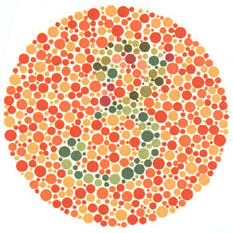
\includegraphics[scale=1.5]{graphics/ishihara.jpg}
	\caption{Ishihara Color Test}
	\label{fig:ishihara}
\end{figure}

The assumption that the movement is simple motivates, in part, the temptation to identify judgements of Sameness with the revolutions of the Circle of the Same. We should not assume that the movement that constitutes the announcement is simple. The Demiurge has fabricated a complex structure for the World Soul. He does so to invest the World Soul with the power of complex motion. The greatness of this power is visibly manifest in the complexity of celestial motion. Notice that the proportional divisions in the substance of the World Soul are not exhaustively used in Timaeus' astronomy. Given the association of the Demiurge and \emph{nous} we can be sure that the the astronomically unused proportions are not there for no reason. Moreover, suppose we follow Aristotle in holding that the soul is the principle of motion and cognition (\emph{De anima} 1 406b28--31). Then it would be plausible that the astronomically unused proportions are cognitively significant. Perhaps the complex motion associated with cognition is sufficiently complex to be discursively structured.


 

% If we abandon that assumption, new interpretative possibilities open up.

% To appreciate this, indulge me in the following speculation. The speculation is offered less as a potential interpretation than as a proof of possibility---a proof that, given the psychogony as Timaeus presents it, the motions of the World Soul are sufficiently complex to be discursively structured by the lights of the \emph{Sophist} account.

% Consider the World Soul applying itself to a divisible being and announcing its character in true opinion. Suppose the World Soul applies itself to Theaetetus and so comes to cognize this divisible being. To cognize Theaeteus is to engage in circular motion. Since it is Theaetetus that is cognized, presumably he is at the center of this circular activity. That is what it means for a divisible being to be the object of cognition. In cognizing Theaetetus, the World Soul recognizes his activity as sitting. To recognize Theaetetus' activity is itself to engage in circular motion. However, since the World Soul is complex, we need not assume that it is the same circular motion as the one that cognizes Theaetetus. Not only has the Demiurge invested the World Soul with a complex structure, He also imposed proportional divisions within its substance. And this opens up the possibility of understanding interweaving within Timaeus's \emph{eikos muthos}. In this case, the proportional divisions of the World Soul are the warp its two revolutions are the weft. Perhaps the two motions are interwoven in the sense that they are harmonious or attuned to the proportional divisions providentially established in the substance of the World Soul. As on Philoponus' take on interweaving, the two circular motions are neither fused nor juxtaposed. They are not fused. The circular motions remain two and the movement constituting the announcement is complex. Nor need they be juxtaposed. Indeed what could juxtaposition even here mean? Interweaving is rather the harmony of their revolutions. On this interpretation, judging the same as the same is the complex motion involving two revolutions attuned to one another. The World Soul's opinion consists in its moving itself throughout its whole being in this complex harmonious fashion. Undoubtedly, the motion is even more complex. The World Soul not only judges thing the same or different, but in what respect, in what manner, when, and where. These must be constituted by either component motions of the complex motion, their properties (such as rate of revolution), or the component motions being appropriately related (such as being attuned in some way).

% The interpretation is not only speculative but incomplete insofar as no specific part of the complex structure has been identified as moving. Nor is it clear how negative statements of inner speech are meant to work. If the components of the complex motion of affirmative statements are concordant, are we to imagine that the components of the complex motion of negative statements are discordant? It is clear that on the model given above this needs to be represented in terms of the proportional divisions within the substance of the World Soul, but how exactly? Despite these limitations, the interpretation illustrates how the Timaean position may be developed once we give up the assumption that the movement is simple. Allowing for the complexity of the World Soul's movement at the very least makes it possible for it be discursively structured.

% section cognition (end)

\section{Knowledge and Opinion} % (fold)
\label{sec:knowledge_and_opinion}

So far, we have been discussing the cognitive activity of the World Soul generally. There are two species of cognitive activity that the World Soul engages in corresponding to its two kinds of objects. The World Soul either applies itself to divisible or indivisible beings. Opinion (\emph{doxa}) and conviction (\emph{pistis}) take divisible beings as their objects, whereas understanding (\emph{nous}) and knowledge (\emph{epistēme}) take indivisible beings as their objects. 

The two species of cognitive activity are not merely distinguished by their objects. It is not just the objects of cognition that distinguish knowledge from opinion, but the character of these acts differ as well. Moreover, the character of the acts differs in three ways. First, opinion and knowledge differ in that they involve the World Soul moving different parts of itself. Second, opinion and knowledge differ in that the movements themselves differ. Third, the resulting cognitive states, opinion and knowledge, are differently described, as true proclamation and disclosure. More explicitly:
\begin{enumerate}[(1)]
	\item Whenever the World Soul takes something sensible from the realm of Becoming as the object of its cognition:
	\begin{enumerate}
		\item the Circle of the Different moves
		\item in a straight course (\emph{orthos})
		\item and proclaims it to the whole soul
	\end{enumerate}
and this is true opinion and conviction.
	\item Whenever the World Soul takes something intelligible as the object of its cognition:
	\begin{enumerate}
		\item the Circle of the Same moves
		\item by spinning truly (\emph{eutroxos})
		\item and thus discloses its object
	\end{enumerate}
and this is understanding and knowledge.
\end{enumerate}

(a) Opinion involves the revolution of the Circle of the Different while knowledge involves the revolution of the Circle of the Same. This is not a reflection of any substantial difference between them. Both are composed of the same mixture of Being, Sameness, and Difference, with the same proportional divisions. Moreover, the World Soul needs to judge the same as the same and the different as different with respect to both the sensible and the intelligible. That the circles are composed of Sameness and Difference allows them to do just that by the principle that like is known by like. If the motion of the different parts is not explained by a substantial difference between them, then why is \emph{doxa} and \emph{pistis} associated with the movement of the Circle of the Different and \emph{nous} and \emph{epistēme} with the the movement of the Circle of the Same?

That the Circle of the Same comprehends the intelligible is a manifestation of the sovereignty granted to it by the Demiurge. It was this sovereignty that allowed the Circle of the Same to remain undivided unlike the Circle of the Different. Perhaps the integrity and order of the seven circles of the Different are sustained by the power and authority of the Circle of the Same whose wisdom derives from contemplating the intelligible. The Circle of the Different is not sovereign but is governed. That it comprehends only the sensible and the corporeal is a manifestation of its inferior status. At least in mortal beings, opinion is connected with \emph{aisthēsis} and the linear motion of \emph{aisthēsis} is the source of turbulence and ethical unrest. It is well that such is governed by the wisdom that contemplating the intelligible brings. The World Soul is not troubled by embodiment the way that the souls of mortal beings are, in part, because it is not embedded in an environment with strong powers. Nevertheless, as elder sister, World Soul exemplifies the cognitive psychology that virtuous mortals must display if they are to face well the ethical challenges of this corporeal life. The motion of the different parts of the World Soul is not explained by a substantial difference between them. There is no substantial difference between the Circles of the Same and the Different. Rather, different parts of the World Soul are moved in knowledge and opinion because the one rules and the other is ruled, an arrangement that is rational, harmonious, and providentially significant.

(b) Opinion and knowledge differ not only in that the World Soul moves different parts of itself, but the movements of the different parts themselves differ. Whereas the Circle of the Different moves in a straight course (\emph{orthos}), the Circle of the Same spins truly (\emph{eutroxos}). This might seem puzzling at first. After all, both are circles, and so both revolve. So in what sense is the course of the Circle of the Different straight? Consider, then, three hypotheses. It is unclear which, if any, apply.

First, motion, for Timaeus, is either circular or linear and there are six forms of linear motion. The oppositional structure here is one--many. Perhaps a complex motion may be more or less circular or more or less linear depending upon the motions from which it is compounded. On the first hypothesis, the Circle of the Different, though it revolves, its motion is complex and involves its circular motion compounding with linear motion. The Circle of the Same, by contrast, is either purely circular or is compounded with significantly less linear motion. This at least seems apt with respect to the mortal counterparts of the World Soul. It might seem natural that the motion of the Circle of the Different, though circular, be compounded with linear motion given the impact of linear \emph{aisthēsis} (the dramatic effects of which are vividly described in the shock of embodiment).

Second, perhaps the straight course of the Circle of the Different is not a matter of being compounded with linear motion so much as an appearance induced by the partial perspective from which its revolution is described. Think of a salient point on one of the circles of the Different. In the visible realm, a wanderer in its orbit would do. The wanderer moves along the path of the revolution of one of the circles of the Different. But from its perspective, it does not revolve so much as it suffers forward motion.  Taken as a whole the circle revolves, in so revolving a part of the circle suffers forward motion. On the second hypothesis, it is a perspective relative aspect of the revolution that is described as straight, rather than a component motion. What is the cognitive significance of this? Perhaps \emph{nous} and \emph{epistēme} are more of a whole than \emph{doxa}, the indivisible Being of their objects making it possible to be more intimately united with them than with the divisible Being of the sensible and the corporeal. Moreover, the Circle of the Different is itself divided into parts. Perhaps the partial perspective from which its activity is described is also a reflection of this as well as the divisible character of its object.

The first two hypotheses share the assumption that moving in a straight course is a distinctive feature of the motion of the Circle of the Different. Perhaps, Timaeus is describing the motion of the Circle of the Different in terms of a general feature that it shares with the motion of the Circle of the Same. Perhaps, Timaeus has in mind what he elsewhere describes as \emph{pros ta auta}, that the motion is always in the same direction. If Timaeus is describing a general feature common to the motions of the Circles of the Same and the Different, then, on this hypothesis at least, he has failed to specify a motion that differentiates \emph{doxa} from \emph{nous}. Perhaps, while the motion of the Circle of the Different does not have a feature that distinguishes it from the motion of the Circle of the Same, the motion of the Circle of the Same has a feature that distinguishes it from the motion of the Circle of the Different. Even if they are not differentiated by their motion, \emph{doxa} and \emph{nous} would remain different species of cognitive activity since they involve the motion of different parts of the World Soul in their apprehension of their different kinds of objects.

If, however, we retain the idea that different species of cognitive activity are associated, not only with different moving parts, but with different motions, then, however we are to understand the contrast, that the motion of the Circle of the Same is somehow more purely circular is appropriate given its sovereignty over the Circle of the Different.

(c) When the World Soul applies itself to a divisible being, it moves the Circle of the Different within. It is the World Soul that in this way opines, and not the Circle of the Different. This is why Timaeus describes the movement of the Circle of the Different as proclaiming the the sensible object to the whole soul. The World Soul is not merely a passive recipient of this proclamation. The whole soul receives the proclamation without speech or sound. But the whole soul does not merely listen, in its way, to the silent proclamation of a part, but it is the whole soul that proclaims and so opines by moving that part. (Compare: It is I, and not my arm, that hails the bus by my arm's movement. It is I, and not my arm, that Thatcher intended to shame for taking a bus beyond the age of 26.) When the Circle of the Different moves, it is the the World Soul that moves a part of itself and so proclaims truly about the sensible and the corporeal. 

When it comes to understanding and knowledge, however, Timaeus shifts the cognitive metaphor. Understanding and knowledge are not so much as proclaimed as revealed. Understanding and knowledge disclose the character of their intelligible objects. What is at stake here is not how the movement of a part may be the activity of the whole so much as the cognitive significance of such movement. The revolution of the Circle of the Same discloses its intelligible object. Timaeus' language, here, is sufficiently striking and dramatic, the Circle of the Same disclosing the intelligible, that proclaiming truly about the sensible seems impoverished by contrast. If opinion is a report, knowledge is an encounter. The former may report the truth, but in the latter the truth is unveiled. Compare the contrast between testimony and first-hand experience. 

A puzzle about the nature of the opinion arises at this point in Timaeus' speech. Opinion is connected with perception. Given that the World Soul has the cognitive power to frame true opinion about the sensible and the corporeal, does that mean that it has the power of perception as well? This can seem unlikely, since the Cosmos has been deprived of the instruments of perception. The Cosmos lacks an environment, and so has no need of the instruments of environmental powers, powers that are only ever exercised in an environment. But perception, or at least the familiar mortal kind, is an environmental power, taking as its object aspects of the environment. This would suggest that the Cosmos lacks perception. But if there is no cosmic perception, then given the connection between \emph{doxa} and \emph{aisthēsis}, how can the World Soul so much as opine about the sensible and the corporeal? It would seem that Timeaus must either:
\begin{enumerate}[(1)]
	\item deny that \emph{doxa} depends upon \emph{aisthēsis} generally, while mortal opinion depends upon perception, cosmic opinion does not, or
	\item deny that \emph{aisthēsis} is an environmental power generally, while mortal perception is environmental, cosmic perception is not. 
\end{enumerate}

Let us briefly consider both alternatives.

First, Timaeus might deny that the Cosmos has perception and maintain that while mortal opinion depends upon perception, cosmic opinion does not. How does mortal opinion depend upon perception? One way that mortal perception contributes to opinion is by identifying the subject of inner speech. One perceives Theaetetus, recognizes that he is sitting, and opines that Theaetetus is sitting, this being proclaimed throughout one's whole soul by the complex and harmonious movement of the Circle of the Different. Theaetetus is the subject of this proclamation and was identified by perception. If the Cosmos lacks perception, how, then, are the subjects of true proclamations identified? One suggestion might be that the subjects of true proclamations are what the World Soul applies itself to. 

This may depend not only upon a cognitive reading of \emph{ephaptētai}, but a particular cognitive reading. Perception is a mode of sensory apprehension. If \emph{ephaptētai} parallels perception in the fixation of Cosmic opinion, then it to must be a mode of apprehension. But it cannot be read as cognitive apprehension (as its occurrence at \emph{Symposium} 212a must be) since \emph{ephaptētai} is less than the whole cognitive act. In response to this difficulty we considered two restricted cognitive readings (section~\ref{sec:_emph_ephatetai}):
\begin{enumerate}[(1)]
	\item \emph{ephaptētai} is a kind of pre-cognitive attentive contact with the object of cognition
	\item \emph{ephaptētai} is kind of reaching out toward the object of cognition, a pre-cognitive orientation toward that object
\end{enumerate}
The first restricted cognitive reading can seem to provide an attractive resolution. The Cosmos lacks perception and so cannot identify by means of perception the subject of its inner speech. But attention, like perception, is a mode of apprehension. If the World Soul may selectively attend to different aspects of the sensible realm of Becoming, then it has the means of identifying the subject of inner speech without perception. The difficulty with this reading was that it is implausible to think that the object of cognition is wholly determined prior to the cognitive act. This motivated the second restricted cognitive reading of \emph{ephaptētai}. The idea is that \emph{ephaptētai} is the process by which the object of cognition is identified and not its identification. The second restricted cognitive reading of \emph{ephaptētai} thus plays a role disanalogous to the role that perception plays in the fixation of mortal opinion. But perhaps this has to do with the difference between mortal and cosmic perspectives. The objects of mortal opinion are external to mortal beings whereas the objects of cosmic opinion are internal to the Cosmos and so require no instruments to identify. 

Second, Timaeus might maintain that opinion depends upon perception quite generally and attribute perception to the Cosmos. The Cosmos lacks an environment and so lacks environmental powers and their instruments. So if the Cosmos has perception, perception must not be environmental generally. While mortal perception is environmental, cosmic perception is not. Proclus (\emph{In Timaeum} 2 83.3–85.31, \citealt{Diehl:1903re}) gives an interpretation of this kind (for a contemporary defence of this Proclean interpretation see \citealt{Reydams-Schils:1997aa}). Allow me to illustrate the second alternative by presenting the Proclean interpretation in terms that we have developed over the course of our discussion.

Proclus claims that cosmic perception differs fundamentally from mortal perception. Mortal perception is environmental. Mortal beings are embodied and embedded in an environment that circumscribes them. The power of mortal perception is only ever exercised in an environment and takes as its object aspects of that environment. Thus a distinction is marked between the perceiver and the object of perception. The Cosmos, while embodied, is not embedded in an environment. Beyond the limits of the Cosmos is neither space nor void. The Cosmos does not have an environment, it is the environment. Thus, if the Cosmos possesses the power of perception, it must not be an environmental power. As Timaeus' arguments about cosmic morphology make clear (33b8–34a8, discussed in chapter~\ref{sec:the_shape_of_the_Cosmos}), the Cosmos has a smooth and even surface since it has no need for the instruments of environmental powers that would disrupt that surface. The Cosmos is also comprehensive (discussed in chapter~\ref{sec:the_comprehensiveness_of_the_Cosmos}). It contains within itself all that is sensible. If the Cosmos perceives Theaetetus sitting, the Cosmos perceives a part of itself. Theaetetus is a fleeting part of the Cosmos, composed of material borrowed from the Cosmos and destined to return, as are all other mortal beings. Cosmic perception is thus a mode of sensory self-awareness that Proclus likens to consciousness (\emph{sunasithēsis}). Cosmic perception is akin to bodily awareness. Just as one may be aware of the configuration and activity of one's limbs without the aid of external observation, the Cosmos is aware of the configuration and activity of its parts. 

Cosmic perception differs from mortal perception. Cosmic perception has no need of instruments to operate in an environment. And no distinction is drawn between perceiver and object of perception. But cosmic perception also differs from mortal perception in a further way, in not being divided into the special senses. Timaeus distinguishes the special senses of mortal beings in terms of the parts of the body in which they receives violent affections from without in the causal process that eventuates in perception (65b–68e). But the Cosmos does not receive violent affections from without. There is nothing without to affect it. That is why it is immune to disease and ageing. Cosmic perception remains undifferentiated because, though embodied, the Cosmos is less involved with corporeality than encosmic beings, not being subject to strong powers from without. 

Cosmic perception, being a general mode of sensory self-awareness, has no need of affection from without. There is nothing sensible without the Cosmos. The Cosmos contains all that is sensible. And so it enjoys a general mode of sensory self-awareness, more unified and superior to the special senses of mortal beings. And it is upon this general mode of sensory self-awareness that cosmic opinion depends. The Proclean resolution is ingenious, but suffers from a lack of textual support, though reflection upon it reveals just how closely it adheres to claims that Timaeus in fact makes.

% section knowledge_and_opinion (end)

\section{The Cognitive Significance of Circular Motion} % (fold)
\label{sec:the_cognitive_significance_of_circular_motion}

Motion is either circular or linear. The opposition is one-many, there being six forms of linear motion. Circular motion is rational, and linear motion is irrational. If the opposition were to figure in a development of the Pythagorean table of opposites, circular motion would be in the superior column. 

But why is circular motion rational? What is the connection between cognition and revolution? While Timaeus clearly presupposes such a connection, he never makes that connection explicit. The connection between cognition and revolution is presupposed in two passages. At 34a3-4 the Demiurge assigns to the body of the Cosmos one of the seven motions associated with \emph{nous} and \emph{phronesis}, circular motion, which Timaeus describes as turning uniformly in the same place within itself. At 40a7--b1 Timaeus claims that the fixed stars revolve and goes on to connect this with their sustained thinking. One of the two motions of the fixed stars is uniform and in the same place, and the fixed stars always think the same thoughts about the same objects. Both passages presuppose that there is a connection between cognition and revolution, but neither passage explains what that connection is (\emph{pace} \citealt[119]{Cornford:1935fk}, see \citealt[72--3]{Lee:1976xs}). Perhaps, Timaeus feels free to presuppose a connection between cognition and circular motion because he is drawing upon and elaborating an Eleatic tradition of linking the two. Indeed the features of the circular motion that Timaeus finds cognitively significant for the most part have antecedents in Parmenides (on Parmenides and Timaeus on circular motion see \citealt{Ballew:1974hw}.)

If we are to understand the connection between cognition and revolution, we should begin by surveying the features that Timaeus ascribes to circular motion. Specifically, circular motion is:
\begin{enumerate}[(1)]
	\item about something (\emph{peri ta auta})
	\item that it is bound to
	\item throughout the whole
	\item uniform (\emph{kata tauta})
	\item in the same place or within its limits (\emph{en tō autō})
	\item in the same direction (\emph{pros ta auta})
\end{enumerate}
These features are not as distinct as their enumeration may suggest. A question to bear in mind as we review these is whether these are features of circular motion generally, or whether at least some of these are features of specific circular motions that Timaeus finds cognitively significant. It will emerge that Timaeus has provided a specific kind of circular motion as a corporeal image of cognitive activity.

(1) \emph{Circular motion is about something (\emph{peri ta auta})}. Circular motion is about or around something. A revolving circle moves round about itself. More specifically, it has a center or central axis around or about which it revolves. This is a general feature of circular motion. 

In the first instance I translated \emph{peri} as about to bring out the connection with the preposition's use to specify the object of cognition (see, for example, 40a7--b1). Just as the circular motion is about something, a center or central axis around which it revolves, thoughts are about their objects.

The pun can be found in Homer, where the body of dead comrade may be fought about (\emph{amphi} or \emph{peri}) both in the sense of the body being the object of the fight and in the sense that it is fought around the body. While the origin of the pun is Homeric, it seems to have enjoyed an Eleatic revival (\citealt[191--3]{Mourelatos:2008ve}). Parmenides maintains that only Being is intelligible. And so only Being is the object of thought. Parmenides conceives of Being as spatially extended and finite, in the shape of a sphere. If the thought that thinks the One Being involves spatial movement, it could only go around that sphere. Thought is about its object by going around it. Thus the unnamed goddess that reveals the Ways of Truth and Mortal Opinion to Parmenides proclaims that her thought is \emph{amphis alētheis}.

While Timaeus agrees with Parmenides that there is a mode of Being that is spatially extended---divisible Being---a crucial difference remains. Timaeus countenances, in addition, a mode of being that is not spatially extended---indivisible Being. This is a post-Parmenidean innovation. Parmenides (the historical Parmenides, not the eponymous character of the dialogue) seems never to have considered the possibility of being without extension.

Timaeus retains this Eleatic pun, despite rejecting the Parmenidean claims upon which it depends. Indivisible beings are the intelligible objects of \emph{nous}. As they are without extension, there is no spatial movement around (\emph{peri}) them, the way there is around the sphere of the One Being on Parmenides' account. Parmenides holds that all objects of thought are spatially extended. Timaeus, by contrast, holds that not all objects of thought are spatially extended and so not all thought so much as could be circular movement around an extended thing.

And yet the Eleatic pun of thought being about (\emph{peri}) its object is retained. There is a shift of sense here. For Parmenides, thought literally moved around its object. That is what made the pun apt. (``It's funny because it is true!'') For Timaeus, however, not all objects of thought are such that thought could move around them. What, then, for Timaeus, makes the Eleatic pun apt? The very fact that it is something different from what it was for Parmenides by itself establishes a shift of sense. And not just in what was meant but perhaps also in the meaning of it. While for Parmenides the spatial connotations of \emph{peri} could be taken literally, for Timaeus they are a metaphor at best, at least when it comes to \emph{nous}.

What, then, for Timaeus, makes the metaphor apt? The object of cognition is what the cognitive act is about. In imagining cognitive activity as spatial movement around its object, the cognitive act circumscribes and encompasses its object. That circular motion encompasses what it moves about describes the relationship between the cognitive act and its object. The imagery, here, persists as a dead metaphor in professional philosophical parlance. The object of cognition is the \emph{content} the cognitive act. The object is the content of the cognitive act only if the cognitive act encompasses that object so as to contain it. 

That circular motion encompasses what it moves about may describe the relationship between the cognitive act and its object, but the fact that it is movement that encompasses the object should not be overlooked. The object of cognition may be the content of the cognitive act insofar as it is encompassed and so contained. But the container is unlike a corporeal container. It is not a body, like a \emph{kratēr}, but an activity. Nor is it a corporeal activity. The sensible is the mark of the corporeal, and the World Soul is insensible. So the cognitive activities of the World Soul are incorporeal activities. The object of cognition is encompassed by the incorporeal activity about it.

(2) \emph{Circular motion is bound to the center around which it revolves.} Of the enumerated features this is perhaps the most implicit. The circular motions of the World Soul and the body of the Cosmos are centripetal. This is perhaps clearest with respect to the body of the Cosmos. The revolution of the Circle of the Same determines the revolution of the fixed stars in the Heavens and this motion extends downwards to the center of the Cosmos \citep[32]{Vlastos:1975aa}. In this way, it governs interior revolutions with different axial rotations, such as the revolutions of the wanderers in the sidereal ecliptic plane as determined by the revolution of the Circle of the Different.

There may also be a hint of it in the World Soul applying itself to its object before moving itself. The verb, \emph{ephaptētai}, can be used to convey \emph{binding}, somehow \emph{fixing} or \emph{holding fast} (Homer, \emph{Odyssey} 22 41). And the binding imagery persists in the tactile uses of the verb such as \emph{laying hands on} (Homer, \emph{Odyssey} 5 348). And in \emph{grasping}, understood as a mode of haptic perception, the perceiver binds their hands to the contours of the body grasped and thereby feels its overall shape and volume. And with respect to the cognitive uses of the verb, it is plausible to think thought is bound to its object. (This might itself be an Eleatic echo, \citealt[192]{Mourelatos:2008ve}.) If it was bound to a different object it would be a different thought. And if it was bound to nothing, it would be no thought at all. In the case of \emph{nous}, that object is only bound when the object is understood. What the verb \emph{ephaptētai} describes is the process which eventuates in the object being bound by \emph{nous}. Moreover, this process is the psychological activity of the soul. It is the soul actively seeking out its object to bind itself to. 

Moreover, binding is a means of assimilation. The soul assimilates to what it binds itself too. Soul's assimilation to the object of its cognition is for mortal beings both an ethical challenge and the means to overcome it. If one binds oneself in thought to the sensible and the corporeal, one thinks only mortal thoughts and one's soul correspondingly becomes mortal to the extent that is possible. However, if one binds oneself in thought to the intelligible and incorporeal, then one thinks only immortal thoughts and one's soul correspondingly becomes immortal to the the extent that is possible (90b--c). And when we observe the revolutions of the Heavens, with rational interest and attention, we may, over time, align the circles in our soul with the circles in the World Soul whose movement is visibly manifest in the celestial revolutions (47a--b). And in hearing, with understanding, rational speech or music, we become attuned to the proportional divisions in the World Soul (47c--e, 67a--c, 80a). The Young Gods providentially provide us with vision and audition so that we have the means to assimilate to the immortal and divine, the World Soul, our elder sister who sets a dignified example for us to emulate.

Is being bound to its center meant to be a general feature of circular motion the way that being around or about something is, or is this a feature of the specific circular motion that Timaeus finds astronomically and psychologically significant? It is not meant as a general feature of circular motion, if only because it is implausible for Timaeus to deny that circular motion may be centrifugal, especially given the use of slings in antiquity. Consider, for example, Xenophon's report, in \emph{Anabasis}, of how the Greek mercenaries sent in aid of Cyrus were regularly harassed by Persian slingers. Homer reports the use of slings, and slings were used by the Assyrians and the Persians as well as the Hebrews. Though the Hellenic Greeks favored close combat over the use of projectiles, they deployed slings as well, and the best Hellenic slingers hailed from Rhodes. 

Slings are swung in a circular fashion, and the forward linear trajectory of their ammunition crucially depends upon their centrifugal motion. In Newtonian mechanics, this assumes a frame of reference that rotates with the ammunition so that, relative to it, the ammunition is stationary. In an inertial frame of reference, by contrast, centrifugal forces need not be postulated to explain the forward trajectory of the ammunition. Release from the centripetal force of the sling and Newton's First Law of Motion would suffice. Thus the rotating frame of reference requires the postulation of centrifugal force in a way that the inertial frame of reference does not. However, the present point is not that centrifugal force is indispensable to explaining slinging a projectile. Rather, the point is that the experience of slinging a projectile is phenomenologically vivid and widely shared and so could provide one with a conception of centrifugal motion.

The ammunition varied, though lead pellets were the most effective. Many are marked with ironic or inflammatory inscriptions. The British Museum has a lead pellet inscribed with {\sbl ΔΕΞΑΙ}, ``Catch!'' (see figure~\ref{fig:dexai}). Thus centrifugal motion is common enough, in Hellenic experience, to be the object of military wit. And Critias, in detailing the forces of Atlantis, counts slingers among their troops (\emph{Critias} 119b). It is implausible, then, to think that Timaeus mistook all circular motion to be centripetal. So being bound to its center is not meant as a general feature of circular motion. Centripetal motion thus must have a special cognitive significance for Timaeus.

\begin{figure}[htbp]
	\centering
		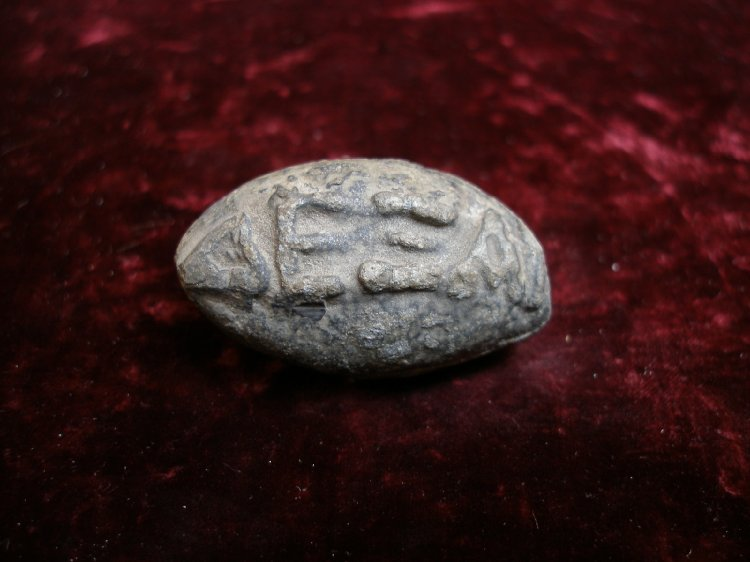
\includegraphics[scale=0.3]{graphics/dexai.jpg}
	\caption{Lead sling bullet with the inscription {\sbl ΔΕΞΑΙ}, ``Catch!'', 4th century BCE, British Museum}
	\label{fig:dexai}
\end{figure}

If being bound to its center is not a general feature of circular motion, then it is a feature of a specific motion that Timaeus finds astronomically and psychologically significant. But what is the cognitive significance of centripetal motion? What is the cognitive significance of the circular motion being bound to its center? By the Eleatic pun, what the motion is about, its center, is what the thought is about, its object. The motion is bound to its center. So, by the Eleatic pun, thought must be bound to its object. Centripetal motion provides us with a corporeal image of cognition, where the soul binds itself to the object that its activity circumscribes and so assimilates to it. Three claims may be distinguished. First binding suggests that the cognitive act and its object are united if distinct. Second, binding suggests that the soul is the agent of the union. Third, that soul binds itself to the object of cognition suggests that the identity of the cognitive act depends upon its object, that with which it unites. The soul's activity submits its identity to its object's determination. And the object determines the identity of the activity so long as that activity persists. This is the means by which the soul assimilates to the object its cognitive activity (90b--c).

While the first feature was a general feature of circular motion, the second was a feature of the specific circular motion that Timaeus finds cognitively significant. Nevertheless, both concern the intentionality of cognitive activity. The first registering the fact that cognitive activity is about something, and so describing the relationship between the cognitive act and its object, and the second describing a feature of that relationship and a consequence of it, that the soul binds itself to the object that its activity circumscribes and so assimilates to it.

(3) \emph{Circular motion is throughout the whole.} There are two separable claims in the vicinity. Both might be in play. First, it might be a claim about agency---it is the whole that moves. Second, it might be a claim about the character of the movement, that it moves as a whole. A third possibility is that Timaeus perhaps intends to combine them in some way. Let us consider these in turn. 

First, perhaps it is the whole that moves. The World Soul applies itself to an indivisible or divisible being and so announces its character throughout the whole of the self-moved. The motion which is the announcement is the self-initiated motion of the whole. When the World Soul applies itself to the object of cognition, it moves itself throughout the whole of its being. This is a claim about the agent of the motion. Even if it is a proper part of the whole that moves, be it the Circle of the Same or the Circle of the Different, in so moving the whole soul moves. In moving the proper part rebels not but its motion is proper to the whole. Cognition is personal. It is the cognizer that cognizes, even if cognizing involves the activity of special parts of the cognizer. The whole soul understands the announcement of the movement of its part because the whole soul is its author.

Second, perhaps the circular motion being throughout the whole is not meant, or at least not merely meant, to be a claim about what moves, the whole. Perhaps, it is also meant as a claim about the character of the motion, that it moves as a whole. Perhaps this is easiest to appreciate with the motion of a whole with divisible parts. So consider five satellites orbiting the Earth. Suppose that they are in the same orbit and maintain a constant rate of revolution so that their radial dimensions remain constant. Just as each individual satellite revolves around the Earth, collectively the satellites revolve around the Earth. But there are differences. An individual satellite may not have completed its period of revolution and so as of yet not revolved around the Earth and yet collectively the satellites have been revolving around the Earth all along. \citet{Lee:1976xs}, following \citet{Vendler:1967ab}, distinguishes between an accomplishment sense of revolution and an activity sense of revolution. The former is divisible into parts. Thus an individual satellite may be one quarter or one half way through its revolution around the Earth. The latter is indivisible. The satellites collectively are simply revolving. There is no sense in which they are half way through their revolutions. The former is only complete when the object circles back to its starting point. The latter is complete at every moment. So while an individual satellite may complete its revolution only once it returns to its starting point, the revolution of the satellites, considered collectively, is complete at every moment. Revolution, in the activity sense, moves as a whole.

Third, perhaps these two ideas may be combined. Suppose that it is the whole that moves. The World Soul in applying itself to the object of cognition moves itself throughout the whole of its being in a complex and harmonious fashion. The whole soul may be the agent of the activity even if it is only a part of the soul that moves, the Circle of the Same or the Different, say. However, even in the case where the whole soul moves a part of itself, that part moves as a whole. If it revolves, it does so in the activity sense of revolution. 


(3) \emph{Circular motion is uniform (\emph{kata tauta}).} Timaeus repeatedly attributes this feature to circular motion (34a3, 36c2, 40a7). Uniformity may be assessed along different dimensions, however. Moreover, uniformity may be meant in more specific and more general ways. What, then, is the intended sense of uniformity? 

If Timaeus has in mind the axial rotation of a circle or a voluminous sphere, then perhaps the main intended sense of uniformity may be its unvarying rate of revolution. Still, along these lines, there will be alternatives. Uniformity might consist, for example, in the constant curvature of the path of revolution. On any such interpretation, uniformity is not a feature of circular motion generally. A motion may have a decreasing rate of revolution or, have a path with inconstant curvature, say, and still be circular, at least by some reasonable standard.

% Uniformity understood as unvarying rate of revolution is a feature of specific circular motions that are astronomically and psychologically significant. However, we should be open to other ways in which circular motion, especially when associated with thought, may be uniform. Relatedly, we should be open to these other ways varying in their generality.

Perhaps, however, Timaeus has in mind a notion of uniformity connected with the movement of a whole. The revolution of the whole revolving itself as a whole is uniform. Since revolution in the activity sense is indivisible, each moment of its revolving is a revolving. The activity is uniformly a revolving throughout the duration of its performance. So understood, this is not a feature of circular motion generally. A motion may be a revolution in the accomplishment, as opposed to the activity sense, say, and still be circular. Should it stop short of a revolution then it would not have been a revolving. And so it is not uniformly a revolving throughout its performance.

So interpreted, uniformity is the dynamic analogue of the uniformity of Parmenides' One Being. Both are a kind of self-similarity. The uniformity of the One Being is its self-similarity throughout the extent of the voluminous sphere. The uniformity of revolution in the activity sense is its self-similarity throughout the duration of its performance.

This might be a deliberate Eleatic echo. Consider the Eleatic pun where what the motion is about, the center, is what the thought is about, its object. The One Being is the intelligible object of thought. It is spherical and so any motion that encompasses it would have to be circular. If further, the motion is revolution in the activity sense, then the uniformity or self-similarity of the One Being is mirrored by the uniformity or self-similarity of the motion that encompasses it. It is plausible that the uniformity of the motion is inherited from the uniformity of what it is about. In revolving as a whole and so in a self-similar fashion, the motion assimilates to its self-similar object. Perhaps only a self-similar motion may encompass the self-similar. Perhaps part of what it is to cognize the uniformity of the One Being is to move uniformly about it.

We have observed Timaeus' tendency to retain the Eleatic pun even while rejecting the Parmenidean claims upon which it rests. In particular, Timaeus countenances indivisible Being, a kind of Being that is not divided around bodies and so not spatially extended. As indivisible beings are without extension, there is no spatial movement around (\emph{peri}) them, the way there is around the sphere of the One Being on Parmenides’ account. According to Timaeus, however, indivisible beings are the intelligible objects of \emph{nous}. So for Timaeus, not all objects of thought are such that thought so much as could move around them. The Eleatic pun is nevertheless retained and so transformed into a cognitive metaphor. 

Perhaps this Timaean tendency is presently in play. Perhaps the Eleatic pun is retained despite rejecting the Parmenidean claims upon which it rests to highlight what is of cognitive significance. If the circular motion is centripetal, and so bound to the object which it is about, perhaps the uniformity of motion is inherited from the unity of the object that it is bound to. Perhaps, then, at least with respect to \emph{nous}, the self-similarity of the cognitive activity is inherited from the self-similarity of its intelligible object. Perhaps, at least with respect to \emph{nous}, the self-similarity of the cognitive activity, is part of what allows it to cognize the self-similarity of its intelligible object. If so, then the principle that like is known by like is not restricted to substantial likeness, such as being alike in being composed of fire. That the activity is self-similar throughout the duration of its performance is not due to the substance of the agent of the activity. It is a formal feature of the activity and a dynamic analogue of a formal feature of indivisible Being. 

The opinable are not perfectly self-similar the way the intelligible are. But perhaps this interpretation can be extended to \emph{doxa} and its objects in the following fashion. The objects of \emph{doxa} are divided around bodies and subject to change. This allows for both spatial and temporal variation in their qualities. So divided beings need not be perfectly self-similar. Suppose, however, that there is more unity to a divided being than being the content of an arbitrary region of the Receptacle. Contrast the region of the Receptacle occupied by an encosmic divided being, the body of the Moon, say, and the corresponding region of the Receptacle in the pre-cosmic chaos, before the Demiurge has imposed form and number (\emph{eidesi kai arithmois} 53b) upon it. The content of the former is a whole in the way that the content of the latter is not. The content of the former, the body of the Moon, a divisible being, is thus correspondingly more uniform than the latter, the content of a Moon-shaped region of the Receptacle in the pre-cosmic chaos. A divided being may be the content of a region of the Receptacle, but its unity imparts an imperfect uniformity to it akin to the self-similarity of the intelligible. Divisible beings, despite being divided around bodies and subject to change, in possessing the kind of unity that they possess, are in a corresponding sense uniform. Extending the interpretation in this way, the revolution of the Circle of the Different is uniform, its activity self-similar, so as to cognize the uniformity of divisible beings, or as much uniformity as divisible beings may aspire to consistent with their impoverished ontological status.

The uniformity (\emph{kata tauta}) of circular motion is regularly linked with its occurring in the same place or within own its limits (\emph{en tō autō}). The senses of these phrases should be coordinate. So we should consider what \emph{en tō autō} could mean before deciding whether \emph{kata tauta} describes the self-similarity of moving as a whole or some other invariant feature, such as the constant rate of revolution or the constant curvature of the path of revolution.

% Moreover, uniformity is repeatedly connected with the next feature, \emph{en tō autō}), that motion is in the same place or within its limits. 

% What is the cognitive significance of the uniformity of circular motion? If the circular motion is centripetal, and so bound to the object which it is about, perhaps the uniformity of motion is inherited from the unity of the object that it is bound to. To have a different uniformity would to be about a different object, and to lack any uniformity at all would signal a failure ot be about anything at all, and so a failure to cognize.

(4) \emph{Circular motion is in the same place or within its limits (\emph{en tō autō}).} This is not a feature of circular motion generally but a restriction on the kind of thing that could be engaged in the relevant kind of circular motion. Not all things subject to circular motion move in such a way that they remain within the limits of their own contours. A cube may rotate and so engage in circular motion, but as it revolves around its axis at least some of its parts move into a space previously unoccupied by the cube. That which revolves within in its own limits is restricted to what mathematicians describe as solids of rotation. Solids of rotation include circles or spheres but are not restricted to these. Any figure that may be fashioned on a lathe or a potter's wheel would count. In general, a solid of rotation is what would result from rotating a plain curve around an axis of rotation. Only such solids of rotation may move within their own contours. So not every kind of circular motion is cognitively significant, only that which revolves within its own limits is.

Again there may be an Eleatic echo here. The One Being of Parmenides is uniform and within its own limits. On the Eleatic pun, a thought about the One Being would involve a uniform motion circumscribing these limits. In being bound to the One, and so regulating its motion to the limits of the One, thought moves within the limits of the intelligible. Again, Timaeus can be read as retaining the cognitive significance of the Eleatic pun while rejecting the Parmenidean claims upon which it rests. The revolution moving within its own limits is an effect of its centripetal character. In being bound to its center it only ever moves within its own limits, limits determined by the center that the movement is bound to. The cognitive significance of moving within its limits is to highlight the center, the object of cognition. Cognitive activity not only encompasses its object but is bound to it. That the soul binds itself to the object of cognition suggests that the identity of the cognitive act depends upon its object and that the object continues to determine the identity of the activity so long as it persists. In being bound to its object, cognitive activity is thus constrained to move within the limits of this encompassment. Only in this way is the cognitive activity about its object.

Revolution in the accomplishment sense, such as a satellite revolving around the Earth, is not within its own limits. The fixed stars revolve around their axis and revolve around the center of the Cosmos, a visible manifestation of the revolution of the Circle of the Same. The first may be revolution in the activity sense, but the second is at best revolution in the accomplishment sense. But revolution in the accomplishment sense is not movement within its limits. In moving along with the revolution of the Circle of the Same, an individual fixed star does not remain in place. Indeed, Timaeus describes it as forward motion. Perhaps the celestial Heavens as a whole revolve within their limits but a part of it, an individual fixed star, does not. The fixed star does not move in place, it traces a circular path through the Heavens. So revolving within its own limits is a movement of the whole and not of an individual part.

Earlier we raised the question whether \emph{kata tauta} describes the self-similarity of moving as a whole or some other invariant feature, such as the constant rate of revolution or the constant curvature of the path of revolution. We observed that however they are best interpreted, \emph{kata tauta} and \emph{en tō autō} should receive coordinate readings given their repeatedly being linked by Timaeus. Coordinate readings can be given to these phrases when read in light of the transformed Eleatic pun. Cognitive activity is about its object by moving as a whole about it. That cognitive activity is understood as movement as whole, as revolution in the activity sense, has the consequence that it is self-similar and within its own limits. The cognitive activity is self-similar in that every moment throughout the duration of the cognitive activity is a cognizing, and it is within its own limits in that the cognitive activity, in being bound to its object, is solely or exhaustively about that object.

(6) \emph{Circular motion is in the same direction (\emph{pros ta auta})}. The object of cognitive activity may help determine the identity of the cognitive act but so too may its direction. At the very least, in the shock of embodiment, Timaeus represents a change in direction as a disruption of cognitive activity. 

Whether this a general feature of circular motion depends on how strict your standards are. If one only thinks of the axial rotation of a circle or voluminous sphere, then it is natural to think that it is, indeed, a general feature of circular motion. But there are other cases. Does the history of the Cosmos remain cyclical despite the Cosmos being repeatedly spun in different directions in the \emph{Politicus} myth? If motion can remain circular while changing direction, by spinning back and forth, then moving in the same direction is not a general feature of circular motion.

That circular motion is in the same direction is independent of many of the other features of circular motion (1--3, 5). (1) Thus a motion may remain about something even if it changes direction. (2) A change of direction is consistent the circular motion being bound to what it moves about (consider the motion of a tether ball). (3) A motion throughout the whole may change direction. (5) A change of direction is consistent with that motion remaining within its limits. What about the fourth feature, uniformity (\emph{kata tauta})? Recall, the uniformity of the circular motion was understood as kind of self-similarity. Moreover this self-similarity was determined by the uniformity or self-similarity of the the object that the cognitive activity is bound to. Moving in the same direction is a dimension of self-similarity or uniformity. So it would seem that moving in the same direction is entailed by the requirement that the motion be uniform.

Moreover, that the circular motion be in the same direction would be entailed by either of our two interpretations of \emph{kata tauta}. Recall, we wondered whether the \emph{kata tauta} was the self-similarity of the movement as a whole or some other invariant feature, such as constant rate of rotation or the constant curvature of the path of revolution. Moving in the same direction is an invariant feature and so would be entailed on the latter interpretation of \emph{kata tauta}. But moving in the same direction is also a dimension of the self-similarity of the movement as a whole and so would be entailed on the former interpretation of \emph{kata tauta} as well. 

I favor the former interpretation where \emph{kata tauta} is the self-similarity of the movement as a whole. On that interpretation, cognitive activity is about its object by moving as whole around it, revolution in the activity sense. Moreover, this movement as whole is self-similar. Every moment throughout the duration of the cognitive activity is a cognizing. We now learn that uniformity of direction is a pre-condition for this. In order for the movement as a whole to be a cognizing, or at least a cognizing of its object, it must maintain its direction. Indeed, Timaeus represents a change of direction as a cognitive disruption. And this may be a clue as to its cognitive significance.  

What is the cognitive significance of moving in the same direction? As Timaeus narrates the shock of embodiment, a change in direction of the Circles of the Same and the Different is due to violent affection from without, the linear impact of \emph{aisthēsis}. Not only may the direction of its motion change, but a circle may cease moving altogether. Change in direction no less than cessation of movement is represented as a cognitive disruption in Timaeus' narration of the traumatic experience of the newly embodied. Cognitive activity is being modeled on movement as a whole in the same direction. Only in this way could a change in direction count as a cognitive disruption. Timaeus is emphasizing the directionality of cognitive activity. Thought runs its course. When disrupted, one looses the train of one's thought. One loses track. One goes off the rails. The movement as whole is uniformly directed around its object. Not just any activity is cognitive activity, only uniformly directed activity as a whole around the object that it is bound to and so within its own limits is cognitive activity.


  


% section the_cognitive_significance_of_circular_motion (end)

\section{Concluding Observations} % (fold)
\label{sec:concluding_observations_cr}

In the previous chapter we discussed the \emph{aporiai} that besets any attempt to understand Timaeus' spatial descriptions literally. Not only does Timaeus offer conflicting spatial descriptions of the soul (as a voluminous sphere, as inner and outer circles), but we saw how each of these descriptions are internally incoherent. But if the spatial attributes of the World Soul cannot be understood literally, neither can Timaeus' attribution of motion to it. But if motion is not narrowly as locmotion, the how are we to understand it? I have suggested that the motion of the World Soul in cognizing indivisible and divisible beings should be understood more broadly as an incorporeal activity, and that its specific features should be understood as describing the cognitive act in relation to its object. Given the \emph{aporiai} of the previous chapter, this is the only remaining interpretive strategy available to us. That strategy gains some credence when we discover the profoundly Eleatic roots of Timaeus' imagery. Though Timaeus departs from the unnamed Goddess (in admitting inextended being, and perhaps in being more optimistic about the cognition of the sensible and the corporeal), nevertheless he can be understood as elaborating and extending Her epistemology.

% section concluding_observations (end)

% chapter cognitive_revolution (end)